\documentclass[a4paper, 12pt]{article}
\usepackage{geometry}
\geometry{a4paper,
total={170mm,257mm},left=2cm,right=2cm,
top=1cm,bottom=2cm}

\usepackage{mathtext}
\usepackage{amsmath}
\usepackage[T2A]{fontenc}
\usepackage[utf8]{inputenc}
\usepackage[english,russian]{babel}
\usepackage{graphicx, float}
\usepackage{tabularx, colortbl}
\usepackage{caption}
\captionsetup{labelsep=period}

\newcommand{\parag}[1]{\paragraph*{#1:}}
\DeclareSymbolFont{T2Aletters}{T2A}{cmr}{m}{it}
\newcounter{Points}
\setcounter{Points}{1}
\newcommand{\point}{\arabic{Points}. \addtocounter{Points}{1}}
\newcolumntype{C}{>{\centering\arraybackslash}X}

\author{Каграманян Артемий, Б01-208}
\date{\today}
\title{Лабораторная работа 2.2.4\\ Определение коэффициента теплопроводности твёрдых тел } 

\begin{document}
\maketitle

\section{Аннотация}
    \textbf{Цель работы:} 1) определение коэффициентов теплопроводности твёрдых тел путём сравнения с теплопроводностью эталонного материала; 2) вычисление относительных тепловых потерь через боковые поверхности по измеренным значениям температуры вдоль радиусов пластинок. 
    
    \textbf{Оборудование:} набор термопар; зеркальный гальванометр; тонкие резиновые прокладки; исследуемые тела; диск из эталонного материала; штангенциркуль.


\section {Теоретическая справка} 
    Количество теплоты $\Delta q$, протекающее за единицу времени через однородную перегородку толщиной $\Delta z$ и площадью S при разности температур $\Delta T$, определяется формулой:
    \begin{equation}
        \Delta q = \kappa S \dfrac{\Delta T}{\Delta z}    
    \end{equation}

    \(\kappa\) - коэффициент теплопроводности. Но этим способом мы пользоваться не будем, потому что результат получится неточным, однако, есть другое решение.

    \begin{figure}[H]
        \centering
        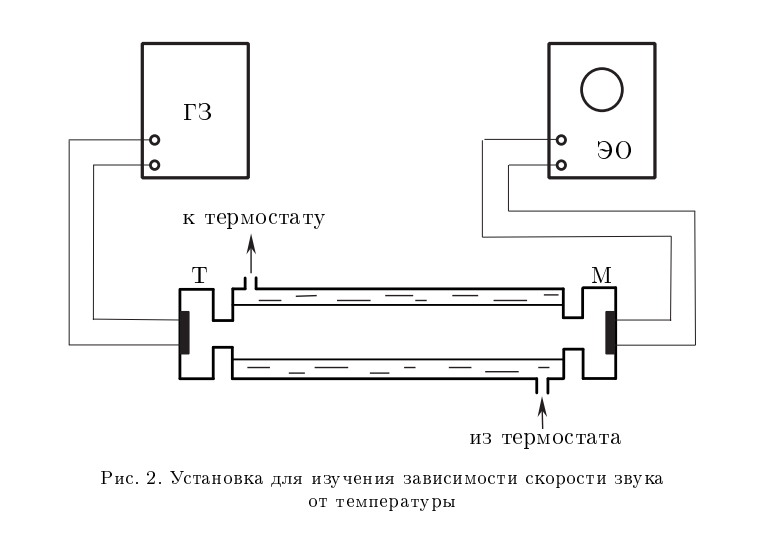
\includegraphics[width=0.7\linewidth]{ust.png}
        \caption{Установка}
    \end{figure}
    
    Две пластинки с коэффициентами теплопроводности $\kappa_1$ и $\kappa_2$ зажимаются между стенками, температуры которых равны $T_1$ и $T_2$ (температуры термостатов). Если  $d_1$ и $d_2$ достаточно малы, то и потери тепла через боковые поверхности тоже малы, тогда:
    \begin{equation}
        \Delta q = \kappa_1 S \dfrac{\Delta T_1}{\Delta z_1} = \kappa_2 S \dfrac{\Delta T_2}{\Delta z_2}
    \end{equation}

    $\Delta z_1 = d_1$ и $\Delta z_2 = d_2$, отсюда:
    \begin{equation}
        \dfrac{\kappa_1}{\kappa_2} = \dfrac{d_1}{d_2} \dfrac{\Delta T_2}{\Delta T_1}
    \end{equation}

    Следует учесть тепловые расходы через боковые стенки пластинок. Полный радиальный поток:
    \begin{equation}
        q_r S_r = - \kappa 2\pi r d \dfrac{dT}{dr}        
    \end{equation}

    Осевой поток:
    \begin{equation}
        q_z S_z = - \kappa \pi r^2 d \dfrac{dT}{dz}        
    \end{equation}

    Отношение данных потоков обозначим за $\delta$ - параметр, который характеризует расширение теплового потока и его относительные потери. Данный параметр не зависит от радиуса:
    \begin{equation}
        \delta = \dfrac{2d \dfrac{dT}{dr}}{r \dfrac{dT}{dz}}        
    \end{equation}
    
\section {Выполнение работы} 
Давайте соберем установку как на картинке и оценим время установления теплового потока через пластинки. Для этого поместим в любое место нашу термопару и построим график зависимости напряжения от времени.

\begin{figure}[H]
        \centering
        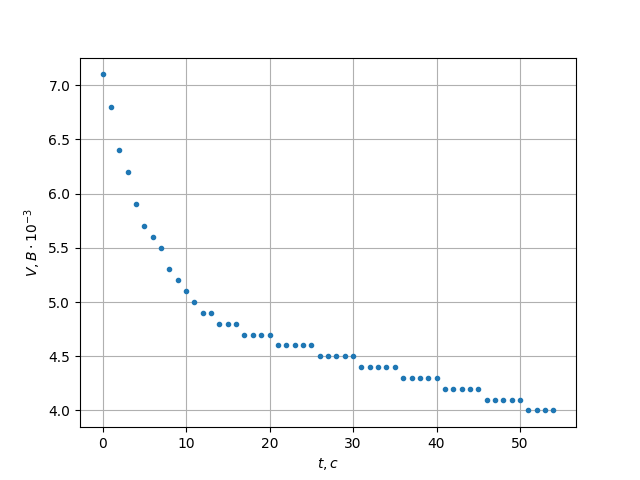
\includegraphics[width=0.8\linewidth]{time.png}
        \caption{Время установления теплового потока}
    \end{figure}

Итого, у нас получилось \(t_{уст} = 54 \ с\). Теперь нам нужно откаллибровать термопары. Для этого разместим их на одном уровне, но оставим расстояние между ними.
Итого, получилось:
\[a_1 = 0,81 \ мВ, \  a_2 = 0,74\ мВ,\ a_3 = 0.88\ мВ,\ a_4 = 0,85\ мВ\]
Далее, отношение разниц температур мы будем считать по формуле:
\[\frac{\Delta T_2}{\Delta T_1} = \frac{U_4/a_4 - U_3/a_3}{U_2/a_2 - U_1/a_1}\]
Дальше нам предстоит измерять теплопроводности разных материалов, помещая в установку разные блины. Вот, что получилось в конце:
\begin{figure}[H]
    \centering
    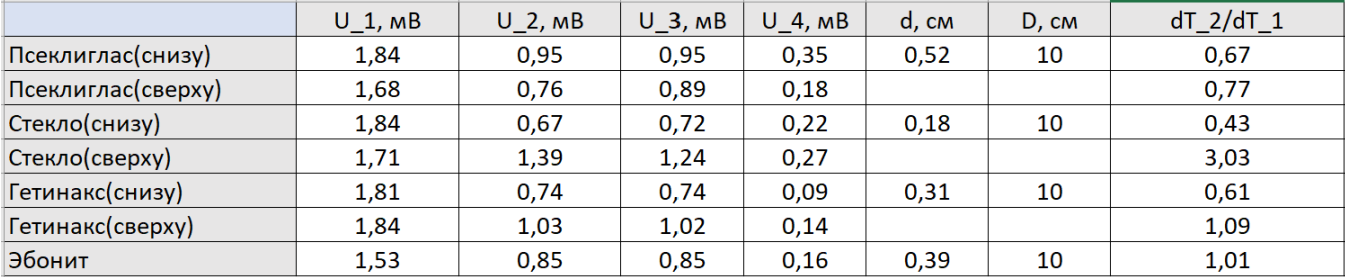
\includegraphics[width=0.9\linewidth]{data.png}
    \caption{Результаты}
\end{figure}

Чтобы убедиться, что наша теория верна, положим 2 эбонитовых блина в установку и измерим отношение теплопроводностей:
\[\dfrac{\kappa_1}{\kappa_2} = \dfrac{d_1}{d_2} \dfrac{\Delta T_2}{\Delta T_1} = 1,018 \pm 0,026 \approx 1\]

Итого, нам осталось посчитать теплопроводности наших материалов и сравнить их с табличными.

\begin{figure}[H]
    \centering
    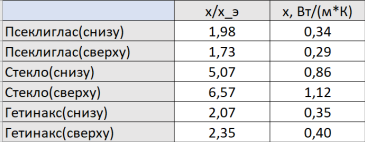
\includegraphics[width=0.5\linewidth]{kappa.png}
    \caption{Теплопроводности}
\end{figure}

Осталось оценить тепловые потери. Расположим термопары так, как показано в описании, и снимем показания:

\begin{figure}[H]
    \centering
    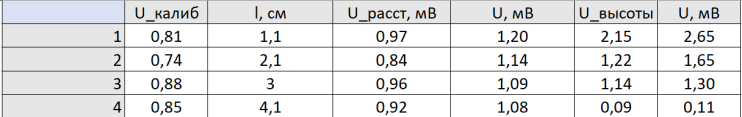
\includegraphics[width=0.8\linewidth]{poteri.png}
\end{figure}

Итого, получилось \(\delta \approx 0.114\)

\section {Заключение}
Мы проделали ряд действий, в результате которых научились измерять теплопроводности разных материалов и оценивать тепловые потери. Все результаты получились сравнимы с табличными в пределах погрешности        
\end{document}
